\documentclass[a4paper, 12pt]{article}        % General format
%\documentclass[a4paper, 14pt]{extarticle}    % Advanced format

%%%% Charset
\usepackage{cmap}                             % Make PDF files searchable and copyable
\usepackage[utf8x]{inputenc}                  % Accept different input encodings
\usepackage[T2A]{fontenc}                     % Russian font
\usepackage[russian]{babel}                   % Multilingual support (T2A)

%%%% Graphics
\usepackage[dvipsnames]{xcolor}               % Driver-independent color extensions
\usepackage{graphicx}                         % Enhanced support for graphics
\usepackage{wrapfig}                          % Produces figures which text can flow around
\usepackage{float}

%%%% Graphs
\usepackage{tikz}                             % Creating graphics programmatically
\usetikzlibrary{arrows}                       % Arrows for tikz

%%%% Math
\usepackage{amsmath}                          % American Mathematical Society (AMS) math facilities
\usepackage{amsfonts}                         % fonts from the AMS
\usepackage{amssymb}                          % additional math symbols

%%%% Typography (don't forget about cm-super)
\usepackage{microtype}                        % subliminal refinements towards typographical perfection
\linespread{1.3}                              % line spacing
\usepackage[left=2.5cm, right=1.5cm, top=2.5cm, bottom=2.5cm]{geometry}
\setlength{\parindent}{0pt}                   % we don't want any paragraph indentation
\usepackage{parskip}                          % add distance between paragraphs

%%%% Tables
\usepackage{tabularx}                         % Enhanced tables
\usepackage{multirow}                         % For tabular
\usepackage{hhline}                           % For tabular

%%%% Other
\usepackage{url}                              % Verbatim with URL-sensitive line breaks
\usepackage{fancyvrb}                         % Sophisticated verbatim text
\setcounter{secnumdepth}{5}                   % Turn on subsection numbering

%------------------------------------------------------------------------------
\usepackage{listings}                         % typeset source code listings

% Цвета для кода
\definecolor{mygreen}{HTML}{3F7F5F}           % color values Red, Green, Blue
\definecolor{mylilas}{RGB}{170,55,241}

% Настройки отображения кода
\lstset{language=Matlab,%
    %basicstyle=\color{red},
    breaklines    =  true,                    % Перенос длинных строк
    morekeywords  =  {matlab2tikz},           %
    keywordstyle  =  \color{blue},            %
    morekeywords  =  [2]{1},                  %
    keywordstyle  =  [2]{\color{black}},      %
    identifierstyle= \color{black},           %
    stringstyle   =  \color{mylilas},         %
    commentstyle  =  \color{mygreen},         %
    showstringspaces=false,                   % don't mark spaces in strings
    frame         =  tblr                     % draw a frame at all sides of the code block
    rulecolor     =  \color{frame},           % Цвет рамки
    tabsize       =  2,                       % tab space width
    showstringspaces=false,                   % don't mark spaces in strings
    numbers       =  left,                    %
    numberstyle   =  {\tiny \color{black}},   % size of the numbers
    numbersep     =  9pt,                     % this defines how far the numbers are from the text
    emph          =  [1]{for,end,break},      %
    emphstyle     =  [1]\color{red},          %some words to emphasise
    %emph         =  [2]{word1,word2},        %
    %emphstyle    =  [2]{style},              %
    extendedchars =  true,                    % Для отображения русского языка
    literate=
        {Ö}{{\"O}}1                    {Ä}{{\"A}}1                    {Ü}{{\"U}}1
        {ß}{{\ss}}1                    {ü}{{\"u}}1                    {ä}{{\"a}}1
        {ö}{{\"o}}1                    {~}{{\textasciitilde}}1        {а}{{\selectfont\char224}}1
        {б}{{\selectfont\char225}}1    {в}{{\selectfont\char226}}1    {г}{{\selectfont\char227}}1
        {д}{{\selectfont\char228}}1    {е}{{\selectfont\char229}}1    {ё}{{\"e}}1
        {ж}{{\selectfont\char230}}1    {з}{{\selectfont\char231}}1    {и}{{\selectfont\char232}}1
        {й}{{\selectfont\char233}}1    {к}{{\selectfont\char234}}1    {л}{{\selectfont\char235}}1
        {м}{{\selectfont\char236}}1    {н}{{\selectfont\char237}}1    {о}{{\selectfont\char238}}1
        {п}{{\selectfont\char239}}1    {р}{{\selectfont\char240}}1    {с}{{\selectfont\char241}}1
        {т}{{\selectfont\char242}}1    {у}{{\selectfont\char243}}1    {ф}{{\selectfont\char244}}1
        {х}{{\selectfont\char245}}1    {ц}{{\selectfont\char246}}1    {ч}{{\selectfont\char247}}1
        {ш}{{\selectfont\char248}}1    {щ}{{\selectfont\char249}}1    {ъ}{{\selectfont\char250}}1
        {ы}{{\selectfont\char251}}1    {ь}{{\selectfont\char252}}1    {э}{{\selectfont\char253}}1
        {ю}{{\selectfont\char254}}1    {я}{{\selectfont\char255}}1    {А}{{\selectfont\char192}}1
        {Б}{{\selectfont\char193}}1    {В}{{\selectfont\char194}}1    {Г}{{\selectfont\char195}}1
        {Д}{{\selectfont\char196}}1    {Е}{{\selectfont\char197}}1    {Ё}{{\"E}}1
        {Ж}{{\selectfont\char198}}1    {З}{{\selectfont\char199}}1    {И}{{\selectfont\char200}}1
        {Й}{{\selectfont\char201}}1    {К}{{\selectfont\char202}}1    {Л}{{\selectfont\char203}}1
        {М}{{\selectfont\char204}}1    {Н}{{\selectfont\char205}}1    {О}{{\selectfont\char206}}1
        {П}{{\selectfont\char207}}1    {Р}{{\selectfont\char208}}1    {С}{{\selectfont\char209}}1
        {Т}{{\selectfont\char210}}1    {У}{{\selectfont\char211}}1    {Ф}{{\selectfont\char212}}1
        {Х}{{\selectfont\char213}}1    {Ц}{{\selectfont\char214}}1    {Ч}{{\selectfont\char215}}1
        {Ш}{{\selectfont\char216}}1    {Щ}{{\selectfont\char217}}1    {Ъ}{{\selectfont\char218}}1
        {Ы}{{\selectfont\char219}}1    {Ь}{{\selectfont\char220}}1    {Э}{{\selectfont\char221}}1
        {Ю}{{\selectfont\char222}}1    {Я}{{\selectfont\char223}}1    {і}{{\selectfont\char105}}1
        {ї}{{\selectfont\char168}}1    {є}{{\selectfont\char185}}1    {ґ}{{\selectfont\char160}}1
        {І}{{\selectfont\char73}}1     {Ї}{{\selectfont\char136}}1    {Є}{{\selectfont\char153}}1
        {Ґ}{{\selectfont\char128}}1
}

\usepackage{caption}                          % Для настройки заголовка кода
\DeclareCaptionFont{white}{\color{сaptiontext}}
\DeclareCaptionFormat{listing}{\parbox{\linewidth}{\colorbox{сaptionbk}{\parbox{\linewidth}{#1#2#3}}\vskip-4pt}}
%\captionsetup[lstlisting]{format=listing,labelfont=white,textfont=white}
\renewcommand{\lstlistingname}{Листинг}       % Переименование Listings в нужное именование структуры
%------------------------------------------------------------------------------

\begin{document}

%------------------------------------------------
\begin{titlepage}
\thispagestyle{empty}

\begin{center}
Санкт-Петербургский политехнический университет Петра Великого\\
Институт компьютерных наук и технологий \\*
Кафедра компьютерных систем и программных технологий \\*
\hrulefill
\end{center}

\vspace{15em}

\begin{center}
\Large Курсовой проект\\по предмету «Проектирование архитектур ПО» \\
\end{center}

\vspace{1em}

% \linebreak
\begin{center}
\textsc{\textbf{Информационная система «Фондовая биржа»}}
\end{center}

\vspace{20em}

\begin{flushleft}
Работу выполнил студент гр. 53501/3 \hrulefill Мартынов С. А. \\
\vspace{1.5em}
Работу принял преподаватель \hrulefill Зозуля А. В. \\
\end{flushleft}

\vspace{\fill}

\begin{center}
Санкт-Петербург \\
2016
\end{center}

\end{titlepage}
%------------------------------------------------
\setcounter{page}{2} % Титульная страница
\tableofcontents

%------------------------------------------------------------------------------

\newpage
\section*{Введение}
\addcontentsline{toc}{section}{Введение}

Информационная система представляет собой сильно упрощенную модель фондовой биржи.

Задачами фондовой биржи в частности является:
\begin{itemize}
\item Предоставление централизованного места, где может происходить как продажа ценных бумаг их первым владельцам, так и вторичная их перепродажа;
\item Выявление равновесной биржевой цены;
\item Обеспечение гласности, открытости биржевых торгов;
\item Установление правил торговли;
\item Обеспечение арбитража;
\item Обеспечение гарантий исполнения сделок;
\item Аккумулирование временно свободных денежных средств и способствование передаче права собственности;
\item Разработка этических стандартов, кодекса поведения участников биржевой торговли.
\end{itemize}

Централизованным местом будет разрабатываемая информационная система, предоставляющая трейдерам возможность выставлять заявки на покупку и продажу инструментов (ценных бумаг). Процесс торговли неизбежно будет формировать выявление равновесной цены. Для обеспечения прозрачности всех процедур, доступ к торговой информации может иметь любой желающий, в то время как проводить сделки (выставлять заявки) могут только авторизованные трейдеры. Трейдер может осуществлять любые сделки в соответствии со своей торговой стратегией, однако пространство арбитража ограниченно одной торговой площадкой, таким образом возможна спекуляция только по времени (при этом биржа естественно не отслеживает портфель инвестора, т.е. он может выставлять на продажу сколько угодно бумаг). Администрация биржи осуществляет управление биржей по средствам установки торговых правил (допуск инструментов, гранулярность) и гарантирует исполнение торговых поручений (с точностью до секунды), в соответствии с правилами. Помимо администрации самой биржи, надзор за торгами имеет ряд контролирующих органов.

За пределами нашего рассмотрения окажутся вопросы аккумулирования денежных средств и передачи прав собственности т.к. это требует построения значительно более сложной модели. Этические стандарты и кодексы поведения так же не будет рассмотрена.

\newpage
\section{Функциональные требования}

Разработать информационную систему «Фондовая биржа», позволяющую организовать процесс продажи и покупки ценных бумаг участниками рынка (трейдерами) с соблюдением требований регулирующий органов.

\subsection{Роли}
Информационная система должна обладать следующими ролями:

\textbf{Администратор биржи} -- осуществляет управление работой биржи, добавляя/удаляя трейдеров и ценные бумаги.

\textbf{Трейдер} -- осуществляет торговлю на бирже, выставляя заявки на продажу и покупку ценных бумаг, отслеживает торговый баланс в рамках торговой сессии.

\textbf{Анонимный пользователь} -- подписывается на рыночную информацию с биржи (чаще всего это строение сервисы, занимающие накопление и анализом рыночных данных для прогнозирования цен).

\textbf{Регулятор} -- осуществляет надзор за работой биржи и может приостановить торги в соответствии со своими внутренними правилами (не всегда эти правила публично доступны а блокировка происходит в случае возникновения подозрений о махинациях или опасных изменениях цены каких-то инструментов).

%\textbf{Биржа} -- исполняет заказы трейдеров и подчиняется правилам администрации и регулятора, рассылает рыночную информацию.

\subsection{Функциональные требования по ролям}

Каждой роле в информационной системе присущи собственные функциональные требования.

\subsubsection{Администратор биржи}
\begin{itemize}
\item авторизация;
\item регистрация нового трейдера (администратор выдаёт логин и пароль);
\item редактирование (в т.ч. изменение статуса блокировки, выставленного администратором) существующего трейдера;
\item регистрация торгового инструмента (ценной бумаги), определение гранулярности торговли;
\item редактирование (в т.ч. изменение статуса блокировки, выставленного администратором) торгового инструмента (ценной бумаги);
\item задание/изменение рамок торговой сессии: аукциона открытия, основных торгов, аукциона закрытия а так же доли биржи от совершения операций;
\item получение/редактирование статуса блокировки биржи (выставляемого администратором);
\end{itemize}

\subsubsection{Трейдер}
\begin{itemize}
\item авторизация;
\item получение статуса работы биржи;
\item получение рыночной информации в рамках торговой сессии и дальнейшие обновления;
\item получение списка торгуемых инструментов;
\item подача/отзыв заявки на покупку/продажу инструмента (включая вид инструмента, цену, объём с учётом гранулярности, срок исполнения);
\item получение торгового баланса в рамках торговой сессии.
\end{itemize}

\subsubsection{Анонимный пользователь}
\begin{itemize}
\item получение статуса работы биржи;
\item получение списка торгуемых инструментов;
\item получение рыночной информации в рамках торговой сессии и дальнейшие обновления.
\end{itemize}

\subsubsection{Регулятор}
\begin{itemize}
\item авторизация;
\item получение рыночной информации в рамках торговой сессии и дальнейшие обновления;
\item получение/редактирование статуса блокировки биржи (выставляемого регулятором);
\item получение/редактирование статуса блокировки ценной бумаги (выставляемого регулятором);
\item получение/редактирование статуса блокировки брокера (выставляемого регулятором);
\end{itemize}

%\subsubsection{Биржа}
%\begin{itemize}
%\item получение/хранение/исполнение заявок от трейдеров;
%\item предоставление списка трейдеров и инструментов администрации и регулятору;
%\item применение правил от администрации и регулятора;
%\item формирование/рассылка/хранение рыночной информации;
%\item ведение и предоставление торгового баланса трейдера в рамках торговой сессии.
%\end{itemize}

\subsection{Прочие требования}

К прочим существенным требованиям относятся

\begin{enumerate}
\item проведение всех операций, подразумевающих создание/редактирование данных требует авторизации;
\item проведение сделок осуществляется по правилу наименьшей цены;
\item точность исполнения заявок -- 1 секунда;
\item отсутствие айсберг-заявок;
\item блокировки могут быть срочными и бессрочными;
\item блокировки администратора и регулятора независимы и работают по правилам дизъюнкции.
\end{enumerate}

\newpage
\section{Варианты использования}

Варианты использования представлены на диаграммах прецедентов (Use Case Diagrams).

\subsection{Администратор биржи}

\begin{figure}[h!]
\centering
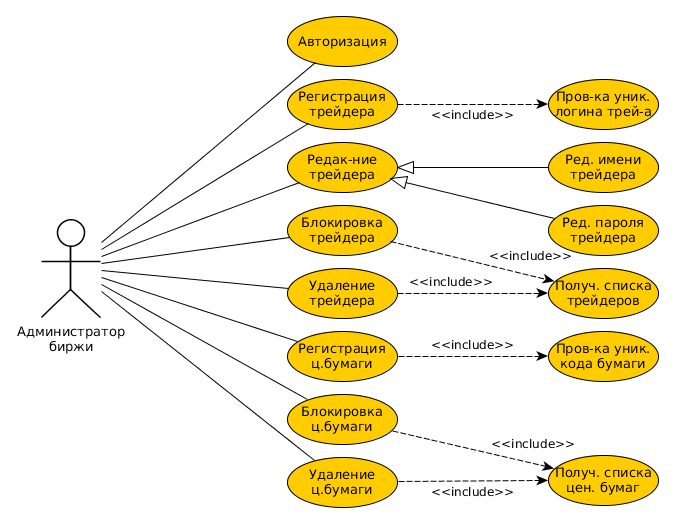
\includegraphics[scale=0.7]{res/pic01}
\caption{Диаграммах прецедентов администратора биржи}
\end{figure}

\subsubsection{Авторизация в программе}

\begin{enumerate}
\item Для того чтобы выполнить вход в систему под пользователем Администратор биржи, необходимо ввести логин и пароль в специальной форме при запуске программы.
\end{enumerate}

Алт.1 Если Пользователь не может выполнить авторизацию как Администратор биржи, он может продолжить работу как Анонимный пользователь.

\subsubsection{Регистрация нового трейдера}

\begin{enumerate}
\item Администратор биржи вводит данные нового трейдера в специальном окне и сохраняет запись
\begin{itemize}
\item (Обязательно) Уникальный логин
\item (Обязательно) Пароль (генерируется администратором)
\item (Обязательно) Имя физического или юридического лица
\item (Опционально) примечания
\end{itemize}
\end{enumerate}

Алт.1 Если администратор биржи не ввёл какое либо из полей или логин не является уникальным, то он получает сообщение об ошибке а новый трейдер не считается созданным.

\subsubsection{Редактирование трейдера}

\begin{enumerate}
\item Администратор биржи получает список трейдеров
\item Администратор изменяет пароль и/или имя и/или примечание трейдера
\item Администратор сохраняет изменения
\end{enumerate}

\subsubsection{Блокирование трейдера}

\begin{enumerate}
\item Администратор биржи получает список трейдеров
\item Администратор выставляет срочную блокировку трейдера (указываю дату и время когда блокировка будет  снята на любой момент в будущем).
\item Администратор сохраняет изменения
\end{enumerate}

Алт.2 Администратор выставляет бессрочную блокировку трейдера (выставляя дату и время снятия блокировки в 0).

Алт.2 Если ранее имелась блокировка, выставленная Администратором, то он может её снять (выставляя дату и время снятия блокировки в любое значение, предшествующее текущему моменту, но не 0).

\subsubsection{Регистрация новой ценной бумаги}

\begin{enumerate}
\item Администратор биржи вводит данные новой ценной бумаги в специальном окне и сохраняет запись
\begin{itemize}
\item (Обязательно) Уникальный код (как правило, 3-5 букв латинского алфавита)
\item (Обязательно) гранулярность торгов
\item (Опционально) примечания
\end{itemize}
\end{enumerate}

Алт.1 Если уникальный код не является уникальным, то Администратор получает сообщение об ошибке а новая ценная бумага не считается созданной.

\subsubsection{Редактирование ценной бумаги}

\begin{enumerate}
\item Администратор биржи получает список ценных бумаг
\item Администратор изменяет гранулярность торгов и/или примечание
\item Администратор сохраняет изменения
\end{enumerate}

\subsubsection{Блокирование ценной бумаги}

\begin{enumerate}
\item Администратор биржи получает список ценных бумаг
\item Администратор выставляет срочную блокировку ценной бумаги (указываю дату и время когда блокировка будет снята на любой момент в будущем).
\item Администратор сохраняет изменения
\end{enumerate}

Алт.2 Администратор выставляет бессрочную блокировку ценной бумаги (выставляя дату и время снятия блокировки в 0).

Алт.2 Если ранее имелась блокировка, выставленная Администратором, то он может её снять (выставляя дату и время снятия блокировки в любое значение, предшествующее текущему моменту, но не 0).

\subsubsection{Задание рамок торговой сессии}

\begin{enumerate}
\item Администратор биржи в специальном окне задаёт время начала и окончания торговой сессии
\item Администратор сохраняет изменения
\end{enumerate}

Алт.2 Если время окончания торговой сессии совпадает или предшествует времени начала, то Администратор получает сообщение об ошибке а данные не сохраняются.

\subsubsection{Задание рамок и условий аукциона открытия}

\begin{enumerate}
\item Администратор биржи в специальном окне отмечает, должны ли применяться правила аукциона открытия
\item Администратор задаёт время окончания аукциона открытия (время начала совпадает с временем начала торговой сессии, а время окончания не может превышать время окончания торговой сессии; время аукциона открытия не должно пересекаться со временем основных торгов и временем аукциона закрытия)
\item Администратор отмечает галочкой, должна ли биржа получать процент с каждой сделки во время аукциона открытия и выставляет этот процент (0 или более)
\item Администратор отмечает галочкой, должна ли биржа получать фиксированную сумму с каждой сделки во время аукциона открытия и выставляет эту фиксированную сумму в копейках (0 или более)
\item Администратор сохраняет изменения
\end{enumerate}

Алт.5 Если введенные данные нарушают ограничения, то Администратор получает сообщение об ошибке а данные не сохраняются.

\subsubsection{Задание рамок и условий основных торгов}

\begin{enumerate}
\item Администратор биржи в специальном окне отмечает, должны ли применяться правила основных торгов
\item Администратор не задаёт время основных торгов (время начала должно превышать время начала торговой сессии, а время окончания не может превышать время окончания торговой сессии; время основных торгов не должно пересекаться со временем аукциона открытия и временем аукциона закрытия)
\item Администратор отмечает галочкой, должна ли биржа получать процент с каждой сделки во время основных торгов и выставляет этот процент (0 или более)
\item Администратор отмечает галочкой, должна ли биржа получать фиксированную сумму с каждой сделки во время основных торгов и выставляет эту фиксированную сумму в копейках (0 или более)
\item Администратор сохраняет изменения
\end{enumerate}

Алт.5 Если введенные данные нарушают ограничения, то Администратор получает сообщение об ошибке а данные не сохраняются.

\subsubsection{Задание рамок и условий аукциона закрытия}

\begin{enumerate}
\item Администратор биржи в специальном окне отмечает, должны ли применяться правила аукциона закрытия
\item Администратор задаёт время открытия аукциона закрытия (время начала должно превышать время начала торговой сессии, а время окончания совпадает со временем окончания торговой сессии; время аукциона закрытия не должно пересекаться со временем аукциона открытия и временем основных торгов)
\item Администратор отмечает галочкой, должна ли биржа получать процент с каждой сделки во время аукциона закрытия и выставляет этот процент (0 или более)
\item Администратор отмечает галочкой, должна ли биржа получать фиксированную сумму с каждой сделки во время аукциона закрытия и выставляет эту фиксированную сумму в копейках (0 или более)
\item Администратор сохраняет изменения
\end{enumerate}

Алт.5 Если введенные данные нарушают ограничения, то Администратор получает сообщение об ошибке а данные не сохраняются.

\subsubsection{Блокирование работы биржи}

\begin{enumerate}
\item Администратор биржи получает статус блокировки биржи
\item Администратор выставляет срочную блокировку биржи (указывая дату и время когда блокировка будет снята на любой момент в будущем).
\item Администратор сохраняет изменения
\end{enumerate}

Алт.2 Администратор выставляет бессрочную блокировку биржи (выставляя дату и время снятия блокировки в 0).

Алт.2 Если ранее имелась блокировка, выставленная Администратором, то он может её снять (выставляя дату и время снятия блокировки в любое значение, предшествующее текущему моменту, но не 0).

\subsection{Трейдер}

\begin{figure}[H]
\centering
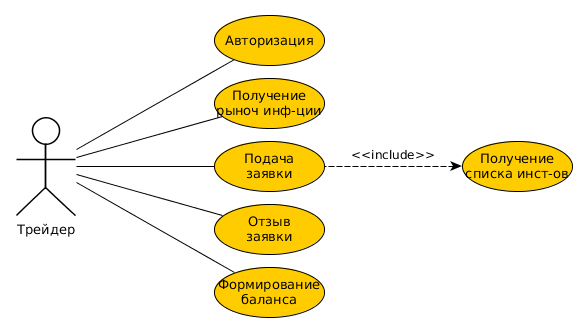
\includegraphics[scale=0.8]{res/pic02}
\caption{Диаграммах прецедентов трейдера}
\end{figure}

\subsubsection{Авторизация в программе}

\begin{enumerate}
\item Для того чтобы выполнить вход в систему под пользователем Трейдер, необходимо ввести логин и пароль в специальной форме при запуске программы.
\end{enumerate}

Алт.1 Если Пользователь не может выполнить авторизацию как Трейдер, он может продолжить работу как Анонимный пользователь.

Алт.1 Если Трейдер блокирован (срочно или бессрочно) Администратором или Регулятором, то он не может завершить регистрацию, но может продолжить работу как Анонимный пользователь.

\subsubsection{Получение статуса работы биржи}

\begin{enumerate}
\item Трейдер отправляет запрос о статусе биржи, и получает статус готовности к работе
\end{enumerate}

Алт.1 Если биржа блокирована (срочно или бессрочно) Администратором или Регулятором, то будет получен статус о неготовности к работе

\subsubsection{Получение списка торгуемых инструментов}

\begin{enumerate}
\item Трейдер получает статус работы биржи
\item Трейдер отправляет запрос о получении списка торгуемых инструментов
\item Трейдер получает списка торгуемых (т.е. не блокированных ни администрацией ни регулятором) инструментов
\end{enumerate}

\subsubsection{Получение рыночной информации}

\begin{enumerate}
\item Трейдер получает статус работы биржи
\item Трейдер отправляет запрос о получении рыночной информации
\item Трейдер получает рыночную информацию с начала торговой сессии до текущего момента
\item Трейдер продолжает получать информацию об обновлении рыночной информации
\end{enumerate}

\subsubsection{Подача заявки на покупку/продажу инструмента}

\begin{enumerate}
\item Трейдер получает статус работы биржи
\item Трейдер получает список торгуемых инструментов
\item Трейдер заполняет заявку и отправляет её на биржу
\begin{itemize}
\item (Обязательно) выбрать ценную бумагу
\item (Обязательно) направление заявки (покупка/продажа)
\item (Обязательно) цена в копейках за 1 бумагу (больше 0)
\item (Обязательно) объём в ценных бумагах, согласно гранулярности биржи (больше 0)
\item (Опционально) время исполнения (больше текущего момента)
\end{itemize}
\end{enumerate}

Алт.3 Если любое обязательное поле не заполнено или гранулярность не совпадает, Трейдер получит сообщение об ошибке, а заявка не будет принята.

\subsubsection{Отзыв заявки на покупку/продажу инструмента}

\begin{enumerate}
\item Трейдер получает статус работы биржи
\item Трейдер получает список своих активных (ещё не исполненных и не отозванных) заявок
\item Трейдер отправляет на биржу заявку с отзывом любой из своих активных заявок
\end{enumerate}

\subsubsection{Получение торгового баланса}

\begin{enumerate}
\item Трейдер получает статус работы биржи
\item Трейдер отправляет на получение торгового баланса с начала торговой сессии
\item Трейдер получает список исполненных заявок и их стоимость
\end{enumerate}

\subsection{Анонимный пользователь}

\begin{figure}[H]
\centering
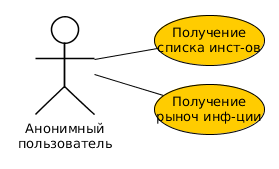
\includegraphics[scale=1]{res/pic03}
\caption{Диаграммах прецедентов анонимного пользователя}
\end{figure}

\subsubsection{Получение статуса работы биржи}

\begin{enumerate}
\item Анонимный пользователь отправляет запрос о статусе биржи, и получает статус готовности к работе
\end{enumerate}

Алт.1 Если биржа блокирована (срочно или бессрочно) Администратором или Регулятором, то будет получен статус о неготовности к работе

\subsubsection{Получение списка торгуемых инструментов}

\begin{enumerate}
\item Анонимный пользователь получает статус работы биржи
\item Анонимный пользователь отправляет запрос о получении списка торгуемых инструментов
\item Анонимный пользователь получает списка торгуемых (т.е. не блокированных ни администрацией ни регулятором) инструментов
\end{enumerate}

\subsubsection{Получение рыночной информации}

\begin{enumerate}
\item Анонимный пользователь получает статус работы биржи
\item Анонимный пользователь отправляет запрос о получении рыночной информации
\item Анонимный пользователь получает рыночную информацию с начала торговой сессии до текущего момента
\item Анонимный пользователь продолжает получать информацию об обновлении рыночной информации
\end{enumerate}

\subsection{Регулятор}

\begin{figure}[H]
\centering
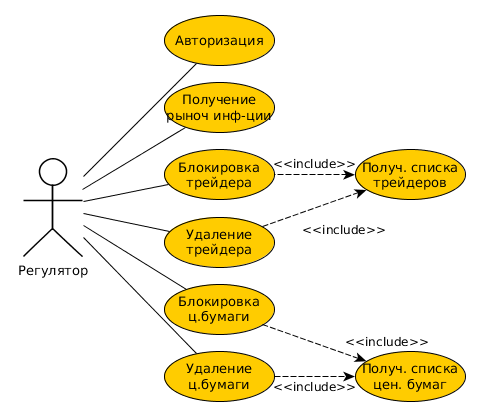
\includegraphics[scale=1]{res/pic04}
\caption{Диаграммах прецедентов регулятора}
\end{figure}

\subsubsection{Авторизация в программе}

\begin{enumerate}
\item Для того чтобы выполнить вход в систему под пользователем Регулятор, необходимо ввести логин и пароль.
\end{enumerate}

Алт.1 Если Пользователь не может выполнить авторизацию как Регулятор, он может продолжить работу как Анонимный пользователь.

\subsubsection{Получение статуса работы биржи}

\begin{enumerate}
\item Регулятор отправляет запрос о статусе биржи, и получает статус готовности к работе
\end{enumerate}

Алт.1 Если биржа блокирована (срочно или бессрочно) Администратором или Регулятором, то будет получен статус о неготовности к работе

\subsubsection{Получение рыночной информации}

\begin{enumerate}
\item Регулятор получает статус работы биржи
\item Регулятор отправляет запрос о получении рыночной информации
\item Регулятор получает рыночную информацию с начала торговой сессии до текущего момента
\item Регулятор продолжает получать информацию об обновлении рыночной информации
\end{enumerate}

\subsubsection{Блокирование работы биржи}

\begin{enumerate}
\item Регулятор биржи получает статус блокировки биржи
\item Регулятор выставляет срочную блокировку биржи (указывая дату и время когда блокировка будет снята на любой момент в будущем).
\item Регулятор сохраняет изменения
\end{enumerate}

Алт.2 Регулятор выставляет бессрочную блокировку биржи (выставляя дату и время снятия блокировки в 0).

Алт.2 Если ранее имелась блокировка, выставленная Регулятором, то он может её снять (выставляя дату и время снятия блокировки в любое значение, предшествующее текущему моменту, но не 0).

\subsubsection{Блокирование трейдера}

\begin{enumerate}
\item Регулятор биржи получает статус блокировки биржи
\item Регулятор биржи получает список трейдеров
\item Регулятор выставляет срочную блокировку трейдера (указывая дату и время когда блокировка будет снята на любой момент в будущем).
\item Регулятор сохраняет изменения
\end{enumerate}

Алт.3 Регулятор выставляет бессрочную блокировку трейдера (выставляя дату и время снятия блокировки в 0).

Алт.3 Если ранее имелась блокировка, выставленная Регулятором, то он может её снять (выставляя дату и время снятия блокировки в любое значение, предшествующее текущему моменту, но не 0).

\subsubsection{Блокирование ценной бумаги}

\begin{enumerate}
\item Регулятор биржи получает статус блокировки биржи
\item Регулятор биржи получает список ценных бумаг
\item Регулятор выставляет срочную блокировку ценной бумаги (указывая дату и время когда блокировка будет снята на любой момент в будущем).
\item Регулятор сохраняет изменения
\end{enumerate}

Алт.3 Регулятор выставляет бессрочную блокировку ценной бумаги (выставляя дату и время снятия блокировки в 0).

Алт.3 Если ранее имелась блокировка, выставленная Регулятором, то он может её снять (выставляя дату и время снятия блокировки в любое значение, предшествующее текущему моменту, но не 0).


\newpage
\section{Статическая модель предметной области}

Статическая модель предметной области представлена диаграммой классов (Static Structure Diagram).

Существуют разные точки зрения на построение диаграмм классов в зависимости от целей их применения:
\begin{itemize}
\item Концептуальная точка зрения -- диаграмма классов описывает модель предметной области, в ней присутствуют только классы прикладных объектов;
\item Точка зрения спецификации -- диаграмма классов применяется при проектировании информационных систем;
\item Точка зрения реализации -- диаграмма классов содержит классы, используемые непосредственно в программном коде (при использовании объектно-ориентированных языков программирования).
\end{itemize}

Реализацию можно автоматически получить из исходного кода. На рисунке 5 представлена реализация слоя сервисов, на рисунке 6 -- слоя инфраструктуры. Отображение более сложных слоёв или сразу нескольких слоём на одной диаграмме затруднительно для понимания.

\begin{figure}[H]
\centering
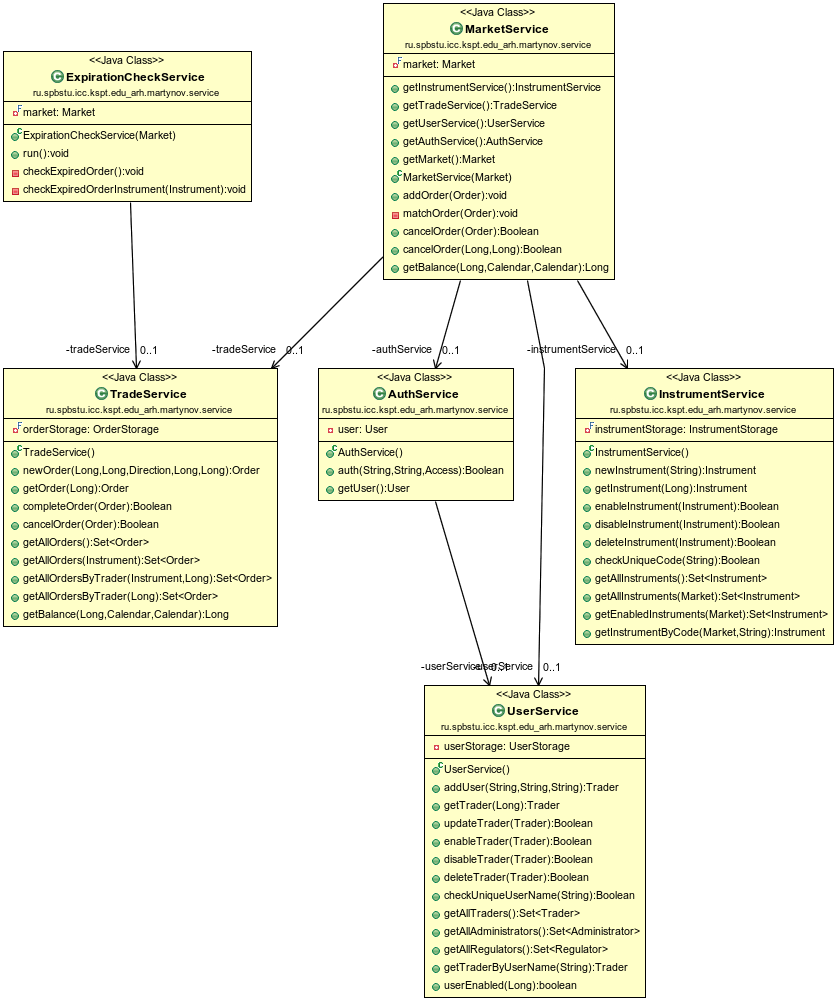
\includegraphics[scale=0.6]{res/pic05}
\caption{Слой сервисов}
\end{figure}

\begin{figure}[H]
\centering
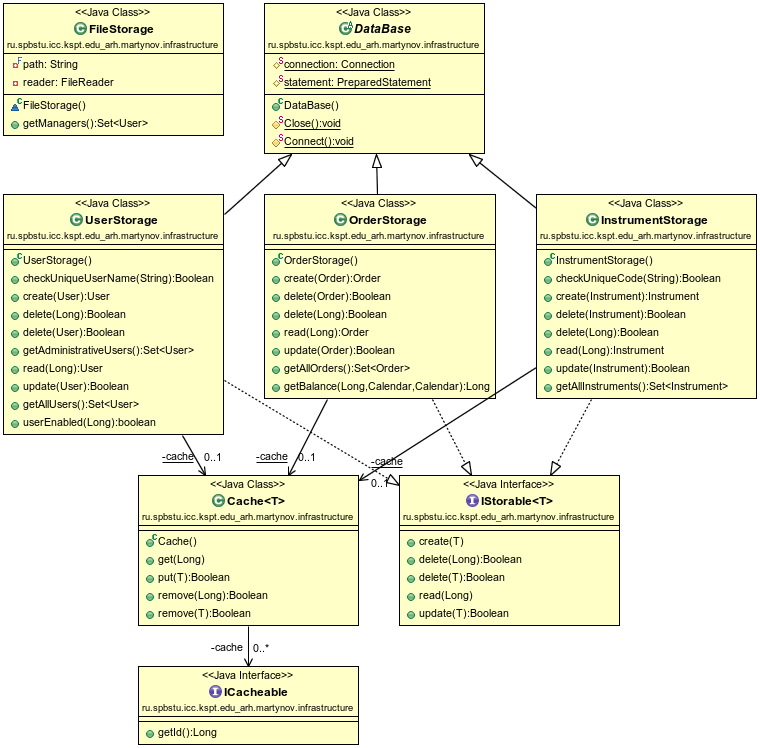
\includegraphics[scale=0.65]{res/pic06}
\caption{Слой инфраструктуры}
\end{figure}

Более общая диаграмма представлена на рисунке 7.

\begin{figure}[H]
\centering
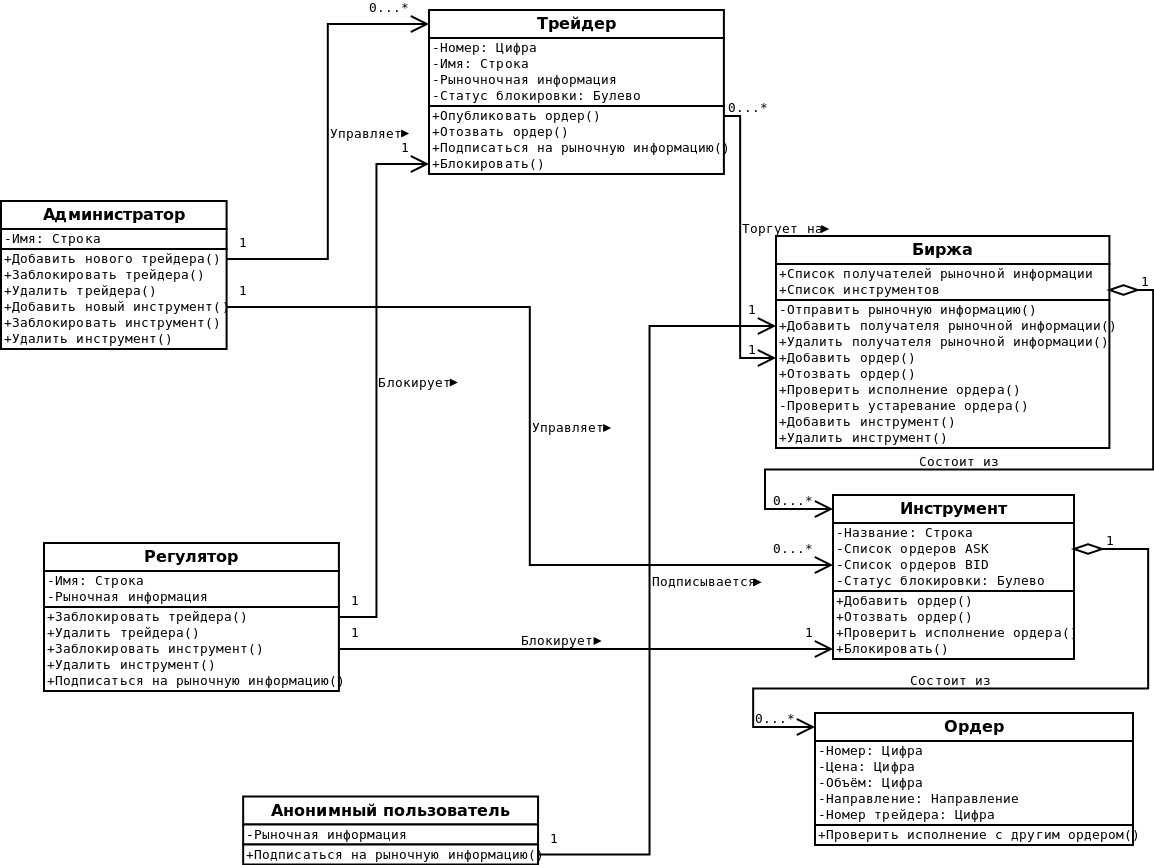
\includegraphics[scale=0.43]{res/pic07}
\caption{Диаграмма классов}
\end{figure}

Анонимный пользоыватель, администратор, регулятор и трейдер имеют общий функкционал -- подписка на рыночную информацию.

Рыночная информация представлена отдельным классом, и состоит из записей MarketRecord. Формат представления соответствует Московской бирже и описывает три события: появление новой заявки, удаление заявки и её выполнение (запись о выполнении будет повторяться два раза т.к. в ней учавствуют две заявки).

Трейдер гененрирует заявки и передаёт их бирже. Биржа раскладывает заявки по инструментам, где они хранятся в виде стакана -- отдельно ask, отдильно bid.

Все исполяемые заявки проходят через клас, определяющий правила торговли. На этом этапе вычисляется доля биржи.

\newpage
\section{Динамическая модель предметной области}

Динамическая модель предметной области представлена диаграммой последовательности (Sequence Diagram).

\begin{figure}[h!]
\centering
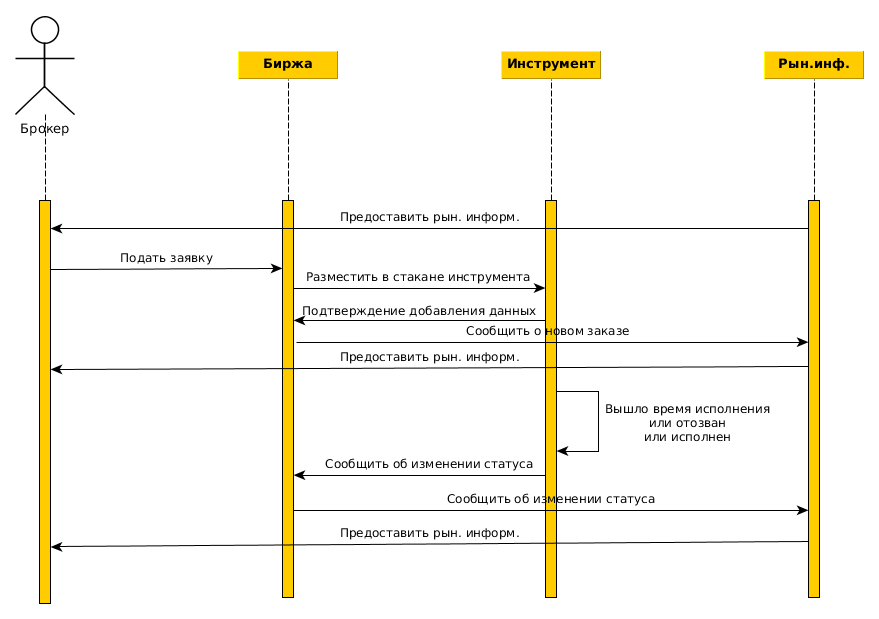
\includegraphics[scale=0.57]{res/pic08}
\caption{диаграммой последовательности заказа}
\end{figure}

Когда брокер формирует новую заявку на покупку или продажу, он передаёт эту заявку на биржу. Биржа хранит заявки по инструментам в стаканах, в зависимости от направления сделки. Как только инструмент принял заявку, информация об этом отображается в Рыночной информации, что могут видеть все участники торгов.

Заявка находися в Инструменте до тех пор, пока её не отзовёт сам брокер, либо не закончится её время исполнения, либо она не будет исполнена.

В любом случае, изменение состояния заявки сразу отображается в рыночной информации (с соответствующим кодом) и об этом сообщается трейдеру, разместившиму заявку.

\newpage
\section{Архитектура приложения}

В процессе работы, архитектура расслоилась на 5 слоёв, взаимодействие которых показано на рисунке 7.

\begin{figure}[h!]
\centering
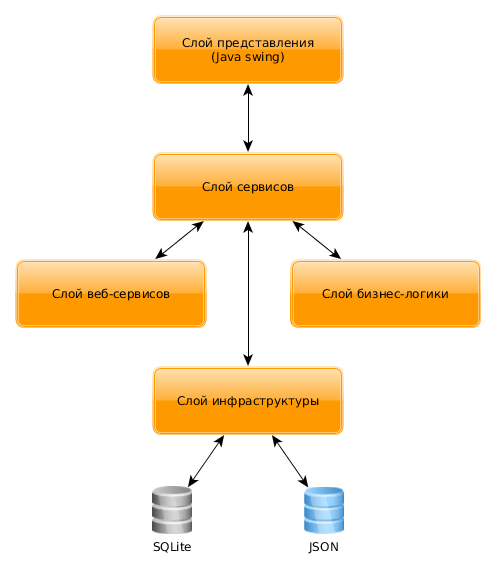
\includegraphics[scale=0.8]{res/pic09}
\caption{Взаимодействие слоёв архитектуры}
\end{figure}

\subsection{Бизнес логика}

В процессе выбора решения по организации бизнес логики были рассмотрены следующие типовые решения:
\begin{itemize}
\item Сценарий транзакции (Transaction Script)
\item Модель предметной области (Domain Model)
\item Модуль таблицы (Table Module)
\end{itemize}

Как подчёркивается в \cite{m1}, рассмотренные решения не являются взаимоисключающими альтернативами и нередко используются совместно для различных частей бизнес логики. Развивая эту идею, работа над реализацией бизнес логики была разделена на на два слабо связанных сегмента: один отвечал за всё конфигурирование биржи, другой за торги.

Конфигурирование биржи фактически сводится к простому сохранению и чтению значений в/из хранилища (базы данных). Тут отсутствуюет какая-то сложная логика, кроме проверки данных на ошибки. Для решения подобных случаев отлично подходит решение Сценарий транзакции.

Торги, напротив, предполагают наличие относительно сложной но однообразной логики, которая затрагивает одновременно большое количество таблиц в базе данных. Кроме того, предметная область требует высокой скорости работы биржи, потому все не завершённые заявки должны постоянно находиться в памяти, что делает этот ресурс сильно востребованым. В этой ситуации наиболее подходящим решением представляется Модуль таблицы.

Между тем, практическая реализация рассмотренных подходов сильно уступала решению Модели предметной области, по крайней мере по части скорости разработки. В \cite{m1} такая ситуация объясняется предыдущим опытом, который имеет разработчик информационной системы. Учитывая, что все типовые варианты взаимозаменяемы, окончательное решение было в пользу Модели предметной области, в той её разновидности, которую сам Фаулер называет "простой", т.е. структура во многом напоминает структуру базы данных.

\subsection{Инфраструктурный слой}

С одной стороны, источником данных в информационной системе является пользователь (трейдер), с другой -- имеется необходимость постоянного хранения рыночной информации и настроек.

В качестве типового решения архитектурны источника данных были рассмотрены следующие:
\begin{itemize}
\item Шлюз таблицы данных (Table Data Gateway)
\item Шлюз записи данных (Row Data Gateway)
\item Активная запись (Active Record)
\item Преобразователь данных (Data Mapper)
\end{itemize}

Фаулер в \cite{m1} приводит таблицу соответствия типовых решений инфраструктурного слоя решениям бизнес-логики. На предыдущем шаге нами было выбрано решение Модель предметной области, таким образом выбор сводился к Активной записи или Преобразователю данных. Шлюз таблицы данных допустимых хоть и допустим, но больше подходит для Модуля таблицы т.к. предоставляет возможности удобной работы с множеством выборок из базы данных (RecordSet). А Шлюз записи данных удобнее всего использовать со Сценарием транзакции т.к. обеспечивает практически сквозую работу с БД, поля объекта есть поля кортежа выборки. Но для выбранной нами Модели предметной области это подходит плохо т.к. сильно увеличивается потребление памяти из-за разрастания представления объектов.

Между Активной записью и Преобразователем данных предпочтение было отдано предпочтение второму. Активная запись хороша, когда к данным хочется добавить логику домена, но в нашем случае вся логика собрана в слое бизнес-логики и сервсином слое. В то же время, было желание максимальной изоляции БД от приложения для лёгкой замены сервера БД -- реляционные базы данных, колоночные, или просто XML-файлы...

\subsection{Сервисный слой}

Были рассмотрены следующие варианты реализации сервисного слоя:
\begin{itemize}
\item Интерфейс доступа к домену (Domain Facade)
\item Сценарий операции (Operation Script)
\end{itemize}

Изначально была выполнена реализация более простого Интерфейса доступа к домену (фактически слой занимался тем, что отдавал рыночные данные и принимал внешние запросы), но это привело к большой сложности в слое бизнес-логики. После этого было принято решение переписать этот слой используя Сценарий операций для разгрузки бизнес-логики.

\subsection{Слой представления}

Слой представления для администратора написан на фреймворке Swing. Он позволяет выполнять базовые операции, согласно функциональным требованиям.

Трейдер тоже имеет свой графический интерфейс, написанный с импользованиемф реймворка Swing, но он имеет минимальную функциональность, и, как правило, имея описание работы протокола многие разработчики предпочитают делать свою реализацию, снобжая её большими аналитическими функциями.

На рисунке 10 представлено окно входа в систему, на рисунке 11 и 12 интерфейст рейдера и регулятора.

\begin{figure}[h!]
\centering
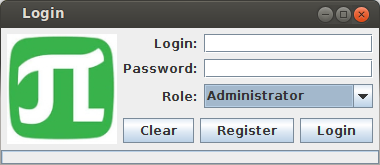
\includegraphics[scale=0.8]{res/pic10}
\caption{Окнов входа в систему}
\end{figure}

\begin{figure}[h!]
\centering
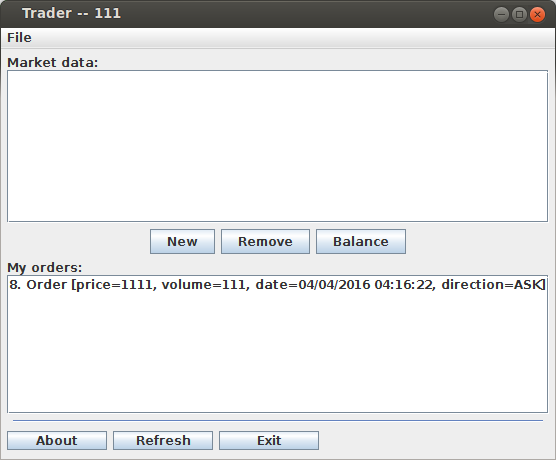
\includegraphics[scale=0.8]{res/pic11}
\caption{Интерфейс трейдера}
\end{figure}

\begin{figure}[H]
\centering
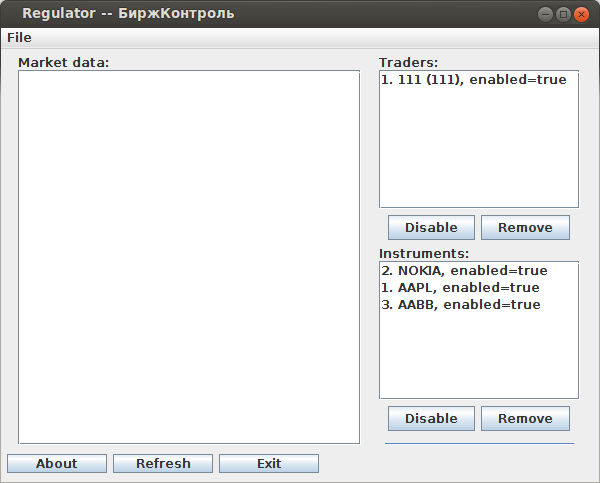
\includegraphics[scale=0.8]{res/pic12}
\caption{Интерфейс регулятора}
\end{figure}

Анонимный пользователь имеют только API. Обычно за ними стоят различные сервисы анализа данных.

\subsection{Слой веб-сервисов}

API для удалённых клиентов реализизовано по средставм простых запросов, релизованных поверх HTTP. Тексовые протоколы не могут обеспечить быстродействие, требуемое в данной предметной области, но они просты и надёжны.

\newpage
\section{Тестирование}

Модульное тестирование, или юнит-тестирование (Unit testing) -- методология тестирования, при которой определенные модули программы тестируются отдельно от остальных модулей. Для выполнения юнит-тестирования в Java наибольшей популярностью пользуется фреймворк под названием Junit4, который мы использовали для тестирования в процессе работы.

JUnit является продуктом  с открытым исходным кодом, и достаточно просто интегрируется со средой разработки Eclipse.

В данной работе мы очень поверхностно использовали возможности данного фреймворка, хотя на реальных проектах он позволяет тестировать большой объём кода и экономить время разработчков.

\begin{figure}[H]
\centering
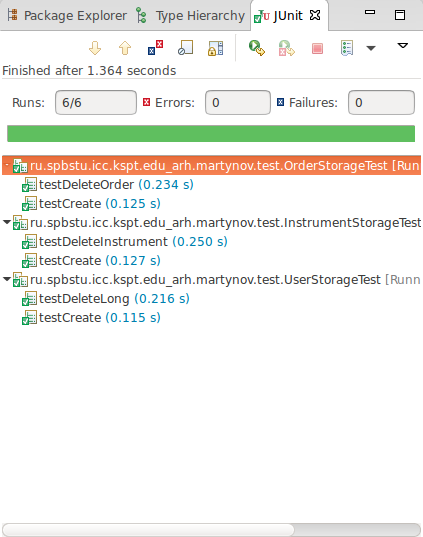
\includegraphics[scale=0.65]{res/pic13}
\caption{Результаты тестирования}
\end{figure}

\newpage
\section*{Заключение}
\addcontentsline{toc}{section}{Заключение}

В результате проектирования системы были изучены различные паттерны проектирование, проведен анализ их возможного использования и в итоге часть из них применена для написания курсовой работы. Были получены навыки проектирования системы от сбора функциональных требований до реализации готового работоспособного приложения,выполняющего требуемые функции. Можно добавить, что знание паттернов проектирования для разработчика является ключевой вещью, т.к. помогает грамотно разрабатывать проекты, повышая эффективность, так же в дальнейшем такие проекты легки для сопровождения.


\newpage
\section*{}
\addcontentsline{toc}{section}{Список литературы}

\begin{thebibliography}{00}

\bibitem{m1} Архитектура корпоративных программных приложений / Фаулер М, Райс Д., Фоммел М. и др. --  Вильямс, 2007 -- 544 с.
\bibitem{m2} Приемы объектно-ориентированного проектирования. Паттерны проектирования / Гамма Э., Хелм Р., Джонсон Р. и др. --   Питер, 2000 -- 366 с.
\end{thebibliography}

%------------------------------------------------------------------------------

\end{document}